\documentclass[3p,times,preprint]{elsarticle}
\newpageafter{author}



%%% Load packages
%\usepackage{amsthm,amsmath}
\usepackage{apalike}
\usepackage{overpic}
\usepackage{diagbox}
\RequirePackage{fix-cm}
%\RequirePackage[authoryear]{natbib}% uncomment this for author-year bibliography
%\RequirePackage{hyperref}
\usepackage[utf8]{inputenc} %unicode support

\abstracttitle{\newpage\hrulefill\newline Abstract}
%\usepackage[applemac]{inputenc} %applemac support if unicode package fails
%\usepackage[latin1]{inputenc} %UNIX support if unicode package fails

\usepackage{tabularx}
\usepackage{siunitx}
\usepackage{titleref}
\usepackage{bchart}
\usepackage{braket} 
\usepackage{nicefrac}
\usepackage{xcolor}
\definecolor{xgreen}{rgb}{0.48,0.84,0.57}
\usepackage{graphicx}
\usepackage{ragged2e}
\usepackage{amsmath,amsfonts}
\usepackage{booktabs} % To thicken table lines
\usepackage{array}
\usepackage{commath}
\newcolumntype{C}{>{\centering\arraybackslash}X}%
\newcolumntype{R}{>{\raggedright\arraybackslash}X}%
\newcolumntype{L}{>{\raggedleft\arraybackslash}X}%

\usepackage{pgffor} 
\usepackage{multirow}

%\usepackage{emoji}
\usepackage{parskip}


\DeclareMathOperator{\sgn}{sgn}
\newcommand{\csentence}[1]{\textbf{#1}.\;} 
\definecolor{coolblack}{rgb}{0, 0, 0.66}
\definecolor{colblack}{rgb}{0.36, 0.54, 0.66}

\definecolor{charcoal}{rgb}{0.21, 0.27, 0.31}
\definecolor{blue}{rgb}{0.0, 0.18, 0.39}
\newcommand{\hideX}[1]{}

%%%%%%%%%%%%%%%%%%%%%%%%%%%%%%%%%%%%%%%%%%%%%%%%%
%%                                             %%
%%  If you wish to display your graphics for   %%
%%  your own use using includegraphic or       %%
%%  includegraphics, then comment out the      %%
%%  following two lines of code.               %%
%%  NB: These line *must* be included when     %%
%%  submitting to BMC.                         %%
%%  All figure files must be submitted as      %%
%%  separate graphics through the BMC          %%
%%  submission process, not included in the    %%
%%  submitted article.                         %%
%%                                             %%
%%%%%%%%%%%%%%%%%%%%%%%%%%%%%%%%%%%%%%%%%%%%%%%%%


%\def\includegraphic{}
%\def\includegraphics{}


\usepackage{etoolbox}


\bibliographystyle{model5-names}\biboptions{authoryear}

%%% Begin ...
\begin{document}

%%% Start of article front matter
\begin{frontmatter}


%% \title{Title\tnoteref{label1}}
%% \tnotetext[label1]{}
%%\author{Name\corref{cor1}\fnref{label2}}
%%\ead{email address}
%% \ead[url]{home page}
%% \fntext[label2]{}
%% \cortext[cor1]{}
%% \address{Address\fnref{label3}}
%% \fntext[label3]{}


\author[santiago]{Germ\'an Lescano}
\ead{gelescano@unse.edu.ar}

\address[santiago]{Instituto de Investigaci\'on en Inform\'atica y Sistemas de Informaci\'on \\Universidad Nacional de Santiago del Estero. Argentina}


\author[cinves]{Jose Torres-Jimenez}
\ead{jtj@cinvestav.mx}
\address[cinves]{Cinvestav Unidad Tamaulipas, Tamaulipas, M\'exico}


\author[santiago]{Rosanna Costaguta}
\ead{costaguta@unse.edu.ar}

\author[conicet]{Anal\'ia Amandi}
\ead{amandi@exa.unicen.edu.ar}
\address[conicet]{N\'ucleo de Inteligencia Comportamental Empresarial, CONICET-UNICEN, Argentina}




\author[cimat]{Carlos Lara\corref{cor1}}
\ead{carlos.lara@cimat.mx}
\address[cimat]{Centro de Investigaci\'on en Matem\'aticas, A.C., M\'exico}

\cortext[cor1]{Corresponding author}



 
 
 


%%%%%%%%%%%%%%%%%%%%%%%%%%%%%%%%%%%%%%%%%%%%%%
%%                                          %%
%% Enter the title of your article here     %%
%%                                          %%
%%%%%%%%%%%%%%%%%%%%%%%%%%%%%%%%%%%%%%%%%%%%%%

\title{Detecting Conflicts in Collaborative Learning through the Valence Change of Atomic Interactions}

%%%%%%%%%%%%%%%%%%%%%%%%%%%%%%%%%%%%%%%%%%%%%%
%%                                          %%
%% Enter the authors here                   %%
%%                                          %%
%% Specify information, if available,       %%
%% in the form:                             %%
%%   <key>={<id1>,<id2>}                    %%
%%   <key>=                                 %%
%% Comment or delete the keys which are     %%
%% not used. Repeat \author command as much %%
%% as required.                             %%
%%                                          %%
%%%%%%%%%%%%%%%%%%%%%%%%%%%%%%%%%%%%%%%%%%%%%%

\newcommand{\hide}[1]{}




%%%%%%%%%%%%%%%%%%%%%%%%%%%%%%%%%%%%%%%%%%%%%%
%%                                          %%
%% The Abstract begins here                 %%
%%                                          %%
%% Please refer to the Instructions for     %%
%% authors on http://www.biomedcentral.com  %%
%% and include the section headings         %%
%% accordingly for your article type.       %%
%%                                          %%
%%%%%%%%%%%%%%%%%%%%%%%%%%%%%%%%%%%%%%%%%%%%%%


\begin{abstract} % abstract
Naturally, every collaboration will bring conflicts that can affect the performance of a team. The earlier a conflict is detected and managed in a collaborative group, the better. Detecting and tracking conflicts in Computer-Supported Collaborative Learning (CSCL) is laborious work. If the teacher does it,  the intervention may be out of time.  Although written dialogues in groups having a conflict reveal the increment of negative emotions in comparison to non-conflict dialogues, a classifier that only uses statistics of the valence of consecutive messages in a  window of the talk shows poor performance. This paper proposes to use features based on the valence change between a message and its response.  In this way the algorithm focuses in the kind of interaction. We study different implementations of the bootstrap aggregating technique to detect conflicts. Results obtained show the viability of the proposed approach.

%\parttitle{First part title} %if any
%Text for this section.
%\parttitle{Second part title} %if any
%Text for this section.
\end{abstract}

%%%%%%%%%%%%%%%%%%%%%%%%%%%%%%%%%%%%%%%%%%%%%%
%%                                          %%
%% The keywords begin here                  %%
%%                                          %%
%% Put each keyword in separate \kwd{}.     %%
%%                                          %%
%%%%%%%%%%%%%%%%%%%%%%%%%%%%%%%%%%%%%%%%%%%%%%

\begin{keyword}
%% keywords here, in the form: keyword \sep keyword
CSCL \sep Conflicts \sep Emotions \sep Sentiment Analysis \sep Bootstrap aggregating

%% MSC codes here, in the form: \MSC code \sep code
%% or \MSC[2008] code \sep code (2000 is the default)

\end{keyword}

% MSC classifications codes, if any
%\begin{keyword}[class=AMS]
%\kwd[Primary ]{}
%\kwd{}
%\kwd[; secondary ]{}
%\end{keyword}

%
%\end{fmbox}% uncomment this for twcolumn layout

\end{frontmatter}

%%%%%%%%%%%%%%%%%%%%%%%%%%%%%%%%%%%%%%%%%%%%%%
%%                                          %%
%% The Main Body begins here                %%
%%                                          %%
%% Please refer to the instructions for     %%
%% authors on:                              %%
%% http://www.biomedcentral.com/info/authors%%
%% and include the section headings         %%
%% accordingly for your article type.       %%
%%                                          %%
%% See the Results and Discussion section   %%
%% for details on how to create sub-sections%%
%%                                          %%
%% use \citep{...} to cite references        %%
%%  \citep{koon} and                         %%
%%  \citep{oreg,khar,zvai,xjon,schn,pond}    %%
%%  \nocite{smith,marg,hunn,advi,koha,mouse}%%
%%                                          %%
%%%%%%%%%%%%%%%%%%%%%%%%%%%%%%%%%%%%%%%%%%%%%%

%%%%%%%%%%%%%%%%%%%%%%%%% start of article main body
% <put your article body there>

%%%%%%%%%%%%%%%%
%% Background %%
%%
\section{Introduction}
\label{intro}
In collaborative learning (CL), students are grouped and paired to achieve an academic goal \citep{gokhale1995collaborative}. In Computer-Supported Collaborative Learning (CSCL), learners interact with the aid of computers. Arranging students in groups and assigning them a task does not guarantee that students will engage effectively \citep{soller2001supporting}. Benefits are mainly observed when the group works correctly. 

\textcolor{coolblack}{
There are plenty of theories and frameworks that support 
collaborative learning. \cite{stahl2020theories} categorize CSCL theories according to the focal unit of collaboration as (i) \textit{subjective theories}, that focus on the individual mind; (ii) \textit{inter-subjective theories},  oriented to social, community, and cultural levels of analysis; and (iii) \textit{inter-objective theories}, that focus on the group itself as the unit of analysis. Even the subjective theories admit that student learning is influenced by the social context.}
Committed groups are composed of participants that encourage other members by asking questions, explaining and justifying their opinions, articulating their reasoning, elaborating, and reflecting on their knowledge \citep{soller2001supporting}. However, interactions that promote learning do not occur spontaneously \citep{onrubia2012role, schwarz2011moderation,tchounikine2010computer}, and the use of computers can even inhibit them \citep{orvis2006computer}.

CSCL groups are exposed to socio-emotional challenges, such as understanding others' perspectives, communication styles, and ways of approaching
teamwork \citep{Jarvenoja2013}. In the interaction between members of a group, conflicts emerge naturally  \citep{Naykki2014}. Conflicts are disagreements between two or more members of the group \citep{Ayoko2008}. Conflicts generate mostly negative emotions and therefore, affects the group work \citep{Dreu2003,Jehn1997,Jiang2013,Lee2015}. %
Conflict resolution depends on the emotional intelligence, social relationships, trust, group cohesion, and social skills manifested by the members \citep{Jiang2013,Kreijns2003,Kwon2014,Lee2015,Rapisarda2002,Slof2016}.

The chat is a common communication channel in CSCL, where participants usually communicate in plain text and emoticons. This channel limits the exchange of emotional expressions because participants cannot perceive gestures or tones of voice of their peers \citep{Feidakis2014}. 
This limitation affects the group's ability to generate cohesion, feelings of trust, belonging, and satisfaction \citep{Nam2014}.  Analogously, it is harder for teachers to recognize the group's emotions, mainly because of the loss of visual contact and acoustic communication. 

Sometimes, teachers want to improve the interpersonal skills of students \citep{Rogat2015,Zheng2016}; for instance, they want to instruct students on conflict management strategies and how they are linked to group performance and satisfaction \citep{Lee2015,Slof2016}. In these cases, it is convenient that the group's activities can generate socio-cognitive or task conflicts \citep{Buchs2004}. Then, the teacher requires to i) identify conflicts,  ii) review the group's interactions following some protocol, and iii) provide feedback that allows students to learn interaction styles \citep{Buchs2004}.

This article addresses the problem of conflict recognition in text interactions. We argue that it is possible to recognize the presence of conflicts through the analysis of the implicit emotions of the text messages. The contribution of this paper is twofold; first, we study the differences in the valence of text messages between conflict and non-conflict situations. Second, we propose a model to recognize conflicts by using statistics of the change of valence between messages and their responses.

The rest of this paper is organized as follows. Section \ref{backgorund} sets out fundamental concepts involved with the subject of study. Section \ref{related} reviews some related literature. Section \ref{detecting} describes the feature extraction from text messages and reviews the bootstrap scheme used for classification. Section \ref{sec:methodology} reveals the research methodology. Section \ref{sec:results} presents the experimental results. Section \ref{disussion} presents a discussion of the work made, and finally, Section \ref{conclusion} concludes this work.

{
\section{Background}\label{backgorund}
\subsection{Conflicts in groups}


Conflicts can be categorized as task and relationship conflicts \citep{Jehn1997}. The former are disagreements regarding opinions, perspectives, and ways of processing the task information
\citep{Ayoko2008,Garcia-Prieto2007,Lee2015}. This type of conflict is positive for the group because it facilitates learning and the development of creative thinking \citep{Jiang2013}, the reevaluation of the status quo, and the elimination of complacency \citep{Ayoko2008}. It promotes innovation, cohesion, commitment, and satisfaction.  It also helps to increase the group performance, levels of understanding, and trust levels among group members  \citep{Dreu2003,Jehn1997,Lee2015,Garcia-Prieto2007}.

Relationship conflicts are disagreements between group members caused by issues unrelated to the task. These conflicts are often manifested as frictions, frustrations, and personality clashes \citep{Ayoko2008,Garcia-Prieto2007,Jehn2001}. This type of conflict generates stress and decreases cohesion, commitment, satisfaction, performance, and quality in decision-making \citep{Naykki2014,Dreu2003,Jehn1997,Lee2015}.
Regardless of the type of conflict, the emotions involved are negative. Negative emotions decrease the capability of working memory, probably by producing an extraneous cognitive load \citep{Dreu2003}. Thus, a substantial increase of negative emotions hamper the group's work \citep{Dreu2003,Jehn1997,Jiang2013,Lee2015}, mainly because of the  dissemination of negative emotions
-- aka emotional contagion \citep{Barsade2009}.

\subsection{Emotions in collaborative learning}
Groups that learn in CSCL environments are exposed to multiple situations that characterize the social dynamic and generate emotions influencing collaborative learning \citep{Jarvela2013}. A typical emotion is frustration \citep{Capdeferro2012}. Emotions in academic environments attract the interest of many researchers; for instance, \cite{Reis2018} consider that the more common emotions are frustration, fear, anger, relaxed, bored, anxious, joy, interested, among others. \cite{Pekrun2002} group academic emotions into four categories: achievement, epistemic,  topic, and social emotions.



Dimensional models of emotions try to describe emotions by their position in two or three dimensions. The bidimensional model describes emotions by their valence (ranging from feeling pleasant to unpleasant) and arousal (ranging from feeling quiet to active) \citep{Coppin2013}. Through these two dimensions, it is possible to describe subjective experiences. Pekrun’s emotion taxonomy \citep{Pekrun2011} is consistent with circumplex models; that is, every affect can be the two-dimensional  (valence/activation) space. %, that is, emotions can be grouped according to their valence and to their degree of activation implied. In terms of valence, positive emotions can be distinguished from negative emotions. In terms of activation, physiologically activating emotions can be differentiated from deactivating emotions.


\subsection{Sentiment Analysis in Text}
%Nowadays, there are tools that enable get the valence or polarity of a sentiment expressed in a text. This allows the technique proposed in this work to be viable to be implemented. Tools to recognize polarity in text can be made with the application of sentiment analysis in text. 
Sentiment analysis tries to find  sentiments and emotions that people express toward products, organizations, people, and other topics \citep{Appel2016,Keshavarz2017,Sanglerdsinlapachai2014}. It is a challenging task because of the ambiguity of words, the complexity of semantic, and the influence of irony, courtesy, writing style, and the language variation among people and culture  \citep{Poria2014}. %Some works made 
Coarse-grained sentiment analysis estimates the valence of a text (positive, negative, or neutral). On the other hand, the fine-grained analysis tries to find the specific emotions. \citep{Giatsoglou2017}. 

 
There are two approaches to detect sentiment in text: (i) the lexical approach uses a ‘lexicon’ to associate words to a given variable; e.g., the intensity of each word \citep{Keshavarz2017}. The result will be the sentiment expressed by the majority of the text words, (ii) the machine learning approach builds a model that recognizes sentiment via the identification of textual patterns \citep{Sanglerdsinlapachai2014}. This model is built by using supervised machine learning, unsupervised machine learning, or a mixed approach. The machine learning approach requires large training data  \citep{Madhoushi2015,Wang2016b}. %Additionally, to these traditional machine learning methods, nowadays, deep learning methods are more applied for sentiment analysis due to the good results obtained regarding to precision, recall, accuracy and F-measure metrics \citep{Yadav2020}.


\section{Related Work}\label{related}
%\cite{Aarnio2013} found that in tutoring groups mediated by computer, cognitive conflicts have low frequency of occurrence and tend to have short duration. This study shows that teachers do not promote  students work their ideas in conflict, and the short duration of conflicts are related with poor skills in argumentation and making questions that activate higher order thoughts. However, \cite{Lao2008} show that the generation of cognitive conflict also depend on the learning methodology applied. \cite{Lao2008} found that Jigsaw technique can generate a major number of cognitive conflicts. Inappropriate use of social skills also drives to intra-group conflicts \citep{Lee2015}.

 \textcolor{coolblack}{Researchers have proposed several features to detect conflicts. } For instance, \cite{Millar1984} study the power dimension of interactions tagged by three alternatives: control gain ($\uparrow$), give up control ($\downarrow$), or neutralize control ($\rightarrow$). They propose that a sequence of three alternative attempts to gain control is a pattern of conflicts.  % The occurrence of this pattern is the first step for a heated exchange of interactions.
% 
The \textit{Interaction Process Analysis} \citep{Bales1950} assigns a tag to each message in a conversation to describe the interlocutors' behavior. 
\cite{Bales1950} states that the tag frequency can be used to infer six types of problems. % Bales (1950) suggests that, in a group without problems, the frequencies of behaviors should be between a lower and upper limit (Tabla \ref{tabla1-bales}).

%propose a methodology to analyze groups called . 

The SYMLOG methodology \citep{Bales1979}  maps  groups and their members into a tridimensional space: dominant/submissive, friendly/unfriendly, and task-oriented/emotional-expressive dimensions. To reveal how frequent specific behaviors happen,  group members should respond to a questionnaire of 26 Likert-questions. \cite{Wall1986}  found that conflicts are not significantly related to the dominant/submissive and the task-oriented/ emotional-expressive dimensions; on the contrary, the friendly/unfriendly dimension is related to conflicts.

To some extent, the friendly/unfriendly  dimension is characterized by the valence dimension of emotions.  Several works \citep{Lescano2020,Wall1986,Zachary1977,Zakaria2009} suggest that the valence of emotions can be used to detect conflicts. Another approach is to detect conflicts via specific emotions; for instance, \cite{Zakaria2009}  suggest that some  negative emotions generate  conflicts (e.g., hate and disgust) and some others (e.g., indifference, misconception, among others) can indirectly predict conflicts. In this work, we show that   negative emotions of interactions can be used to recognize the presence of conflicts in CSCL environments.


\textcolor{coolblack}{The graph-based approaches to conflict detection build a graph that represents relationships between users.  \cite{Zachary1977}  uses social network techniques to identify fission in a group. Fission is a phenomenon about subgroup formation due to the differences in the way sentiments are shared. \cite{Lescano2020} propose to calculate the commute times of a normalized graph in which edges represent the members’ emotional interactions.}%, taking into account bidirectional negative messages in the same conversation thread. They represent chat interactions as a digraph in which the nodes represent users and the edges indicate the transference of negative sentiments during the interactions. Then, a matrix of scaled commute times is used to detect clusters which represent subgroups having conflict.

There are other approaches to recognize conflicts, but they impose restrictions on the interface. For instance, % Tedesco
\cite{Tedesco2003} proposes a framework based on Belief–Desire–Intention logic (BDI logic) that allows recognizing and mediating conflicts in group planning interactions. % Monteserin et al.
\cite{Monteserin2010} define an argumentation plan as a process during a given negotiation; hence, they model the plan as a partial order sequence of arguments that allows students to reach an expected agreement. Their approach offers students assistance inspired by BDI agents \citep{rao1995bdi}. In contrast, the proposed approach does not impose restrictions on the interface, because it can be used to detect automatically conflicts in CSCL chats.

}

\section{An Algorithm to Detect Conflicts in Collaborative Groups} \label{detecting}

This section describes the \textit{Bagging Algorithm to Recognize Conflicts in Groups using Sentiments} (BARCIGUS), a technique based on supervised machine learning to detect conflicts in CSCL group interactions by considering the change of valence between messages.


%In section 4.1 we describe constructs created to explain the technique. Section 4.2 presents the procedure proposed to extract features to train a machine learning model. Finally, in section 4.3, the machine learning algorithm used to build the model is described. 


\subsection{Preliminaries}
A \textit{sequence}, $S$, is an enumerated collection of objects in which repetitions are allowed and order matters. A \textit{subsequence} $S'$ of $S$ is defined as any series of elements that can be obtained from a given sequence $S$ by deleting some of its elements. Let $D = S\setminus S'$ be the subsequence of elements removed from $S$ to obtain $S'$. A sequence $T$ is a supersequence of $S$, if $T$ can be obtained by inserting elements into $S$. In a \textit{contiguous subsequence} or \textit{interval}, the elements (taken in order) are consecutive in the original sequence. A contiguous supersequence of $S$ can be obtained by inserting elements at the beginning or end of $S$.

Let $X$ be a discrete random variable with a range ${x_0,x_1,..., x_{J-1}}$. The  Probability Mass Function (PMF) gives the probability that the discrete random variable is exactly equal to some value. We write $p_X(x_i)$ to represent the probability that the random variable $X$ equals $x_i$, $P(X=x_i)$. The joint probability distribution of two discrete random variables $X$, $Y$ is denoted as $p_{XY}(x,y) = P(X=x,Y=y)$.  For two independent variables $p_{XY}(x,y) = p(x)p(y)$.

The \textit{averaging operation} combines   $m$ discrete random variables into a single discrete random variable. Let us denote as $C = \mathrm{avg} (X_{0},X_{1},\dots, X_{m-1})$ the average of random variables $X_{0},X_{1},\dots, X_{m-1}$. The PMF of $C$ is simply the normalized sum of the input densities, that is
%
\begin{equation}
    p_C(x_i) = \frac{p_{X_0}(x_i) + p_{X_1}(x_i)  + \ldots + p_{X_{m-1}}(x_i)}
    {\sum_{\forall x_j} \left[ p_{X_0}(x_j) + p_{X_1}(x_j)  + \ldots + p_{X_{n-1}}(x_j)\right]} = \frac{\sum_{j}  p_{X_j}(x_i)}{ m}.
\end{equation}.%




\subsection{Features Extraction}

Our main hypothesis is that text messages between participants in a chat could give enough information to detect conflicts. Specifically, we analyze the emotional content of text messages. Thus, the interaction of participants can be characterized by the valence of their messages.

Consider a sequence of $n$ text  messages 
among participants $U$ within a temporal window,
\begin{equation}
M = [\mu_0^{s_0,r_0}, \mu_1^{{s_1,r_1}}, \mu_2^{s_2,r_2}, \ldots, \mu_{n-1}^{s_{n-1},r_{n-1}}] = \left[\mu_i^{s_i,r_i}\right]_{i\in \set{0,\ldots, n-1}}
\end{equation}
where, $\mu_i^{s_i,r_i}$ is a single text message, $i$ is the number of the message, $s_i \in U$ is the sender, $r_i \in U \cup \set{*}$ is the receiver, $s_i \neq r_i$; here, a message to all participants is represented by $*$. 

Let $I^{p,q} = I^{q,p}$ be the interaction set between $p$ and $q$, where $\mu_i^{s_i,r_i} \in I^{p,q}$ is a single message between participants $p$ and $q$; that is, $s_i \in  \set{p,q}$ and   $r_i \in \set{p,q,*}$. The \textit{interaction list} $M^{p,q}$ between two participants $p$ and $q$ is defined as a subsequence of $M$ that contains all messages exchanged between $p$ and $q$ in a given window; formally, %
\begin{equation}
(\mu \in I^{p,q}, \; \forall \mu \in M^{p,q})  \text{ and }  (\mu \not\in I^{p,q}, \; \forall \mu \in M \setminus M^{p,q}).
\end{equation} %


A \textit{two-way interval}, $T=S^p|S^q$, is a contiguous subsequence (interval)  of an interaction list between any two participants $p$ and $q$, that can be represented as a concatenation of two intervals $S^p$ and $S^q$ composed of messages sent by the same participant; i.e., messages of $S^r$ are all sent by the participant $r \in \set{p,q}$ and the receiver is $r \setminus \set{p,q} \cup \set{*}$ .
An \textit{atomic interaction}, $\mathit{A}$, is a two-way interval that does not have a contiguous supersequence forming a two-way interval.

Let $B=\set{-,0,+}$ be the set of sentiment classes (negative, neutral, and positive), and  $\mathcal{C}_T$ be a message-level classifier (e.g., an automated classifier or evaluation by experts) that assigns a PMF on $B$ to each \mbox{message $\mu$.}
%
%To obtain the probability distribution of a two way interval $T=S^p|S^q$, we first combine the distributions of each interval $S^r$ with $r\in\set{p,q}$.

Consider the interval $S^r = [\mu_{r_0},\mu_{r_1}, \ldots \mu_{r_{n-1}}]$ of messages sent by participant $r \in  \set{p,q}$. Let $X_{r_i}$ be the random variable obtained by the classifier $C_T$ from $\mu_{r_i}$. To obtain the PMF of $S^r$ we use the averaging operation, \mbox{$S^r \sim \mathrm{avg}(X_{r_0}, X_{r_1}, \ldots, X_{r_{n-1}})$; } that is,
%
\begin{equation}
    p_{S_r}(b_i) = \frac{\sum_j p_{X_j}(b_i)}
    {n},
\end{equation}%
where $n$ is the number of messages in the interval $S^r$.

By considering independence of intervals $S^p$ and $S^q$, the joint probability distribution of the atomic interaction $A=S^p|S^q$ is%
\begin{equation}
p_A(b_1,b_2) = p_{S^p}(b_1)p_{S^q}(b_2) \;\;\;\; \text{for all  } b_1, b_2 \in B
\end{equation}

To obtain the features of a temporal window $M$, the proposed approach finds the set $\mathbf{A}_M$ of all atomic interactions \mbox{of $M$.} The features of the window, $f(M) \in \mathrm{R}^9$, are found by averaging the PMF of atomic interactions in $\mathbf{A}_M$; that is, $f(M) = \mathrm{avg} ( \mathbf{A}_M)$, the features of the window are used as inputs for the classifier. The complete feature extraction process is exemplified in Fig. \ref{fig:features}.

\newcommand{\MID}{\;\big\vert \;}



\begin{figure}[t!]
    \centering
    \setlength\tabcolsep{2pt}
    \renewcommand{\arraystretch}{1.15}
    \begin{tabularx}{0.98\textwidth}{XXXXp{0.4cm}>{\centering\arraybackslash}p{3.8cm}p{0.4cm}}
    %% ROW
    \multicolumn{4}{c}{\small{
\setlength\tabcolsep{4pt}
\begin{tabularx}{0.63\textwidth}{llllX}
\toprule
msg ID & $i$ & $s_i$ & $r_i$ & Interaction Text\\
\midrule
$\mu_0^{1,2} $  &0& $u_1$ & $u_2$ & bueno y ahora ¿qué leo? \\
$\mu_1^{3,*} $  &1& $u_3$ & * & nosotras tenemos que leer Gardner, inteligencia múltiples  \\
$\mu_2^{1,3} $  &2& $u_1$ & $u_3$  & eso estaba leyendo y me dijeron que no  \\
$\mu_3^{2,1} $  &3& $u_2$ & $u_1$ & Si, no sé, léamos éso porque la verdad no entiendo a la profe \\
$\mu_4^{1,2} $  &4& $u_1$ & $u_2$ & yo tampoco entendí  \\
$\mu_5^{3,*} $  &5& $u_3$ & * & si,  sé qué tenemos que leer, pero del texto que nos dió la profe...\\ 
$\mu_6^{3,*} $  &6& $u_3$ & * & habla de muchos autores  \\  
%$\mu_7^{1,*} $  &7& $u_1$ & * & me duele la cabeza} \\  
\bottomrule
\end{tabularx}
}} 
    &{\Large$\Rightarrow$}
    &{
    \footnotesize
    \renewcommand{\arraystretch}{1.5}
    \begin{tabular}[t!]{llll}
     \toprule
     msg ID&p(+)&p(-)&p(0)\\
     \midrule
       $\mu_0^{1,2}$ &  0.02 & 0.01 & 0.97 \\
       $\mu_1^{3,*}$ &  0.01 & 0.04 & 0.95 \\ 
       $\mu_2^{1,3}$ &  0.00 & 0.97 & 0.03 \\ 
       $\mu_3^{2,1}$ &  0.00 & 0.99 & 0.01 \\ 
       $\mu_4^{1,2}$ &  0.01 & 0.22 & 0.77 \\
       $\mu_5^{3,*}$ &  0.01 & 0.44 & 0.55 \\
       $\mu_6^{3,*}$ &  0.04 & 0.04 & 0.92 \\ 
       $\mu_7^{1,*}$ &  0.00 & 1.00 & 0.00\\
     \bottomrule
     \end{tabular} 
     }
    &{\Large$\Rightarrow$}
    \\
    %% ROW
    \multicolumn{4}{c}{\rule{0pt}{14pt}(a)}
    & &
    (b)\\
    %% ROW
    \\
    %% ROW
    \multicolumn{4}{c}{
    \begin{tabular}{lp{0.4cm}l}
      \toprule
      users & & interaction list \\
      \midrule
        $u_1,u_2$ & &  $M^{1,2}: [\mu_0^{1,2},\;\mu_3^{2,1},
        \; \mu_4^{1,2},\;\mu_7^{1,*}]$ \\
        $u_1,u_3$ & &
        $M^{1,3}: [\mu_1^{3,*}, \; \mu^2_{1,3}, \;  \mu_5^{3,*}, \; \mu_6^{3,*}]$ \\
        $u_2,u_3$ & &
        $M^{2,3}: [\mu_1^{3,*}, \; \mu_5^{3,*}, \; \mu_6^{3,*}]$ \\
      \bottomrule
    \end{tabular}
    }
    &{\Large$\Rightarrow$}
    &
    %% ROW
    {
    \begin{tabular}{lp{0.3cm}l}
      \toprule
      users & &atomic int. \\
      \midrule
        $u_1,u_2$ & &$A_1:\mu_0^{1,2} \mid \mu_3^{2,1}$ \\
        & & $A_2:\mu_3^{2,1} \mid \mu_4^{1,2},\mu^7_{1,*}$ \\
        \midrule
        $u_1,u_3$ & &
        $A_3:\mu_1^{3,*} \mid \mu_2^{1,3}$ \\
         & &
        $A_4:\mu_2^{1,3} \mid  \mu_5^{3,*},\mu_6^{3,*}$ \\
      \bottomrule
    \end{tabular}
    }
    &{\Large$\Rightarrow$}\\
    
    %% ROW
    \multicolumn{4}{c}{(c)}
    & &
    \rule{0pt}{14pt}(d)\\
    %% ROW
     \\
    %% ROW
    {
     \footnotesize
    \begin{tabular}[t!]{lccc}

     & \multicolumn{3}{c}{$S^2$}\\
     \cmidrule{2-4}
    $S^1$ & $+$ & $-$ & $0$  \\
     \midrule
    $+$ & 0.00 & 0.02 & 0.00\\
    $-$ & 0.00 & 0.01 & 0.00\\
    $0$ & 0.00 & 0.96 & 0.01\\
     \midrule
          \multicolumn{4}{c}{$A_1:\mu_0^{1,2} \MID  \mu_3^{2,1}$}\\

     \end{tabular}
     }
     &{
     \footnotesize
    \begin{tabular}[t!]{lccc}
     & \multicolumn{3}{c}{$S^1$}\\
     \cmidrule{2-4}
    $S^2$ & $+$ & $-$ & $0$  \\
     \midrule
    $+$ & 0.00 & 0.00 & 0.00\\
    $-$ & 0.00 & 0.60 & 0.39\\
    $0$ & 0.00 & 0.01 & 0.00\\
     \midrule
     \multicolumn{4}{c}{$A_2:\mu_3^{2,1} \MID  \mu_4^{1,2},\mu_7^{1,*} $}\\

     \end{tabular}
     }
     &{
     \footnotesize
    \begin{tabular}[t!]{lccc}
     & \multicolumn{3}{c}{$S^1$}\\
     \cmidrule{2-4}
   $S^3$ & $+$ & $-$ & $0$  \\
\midrule
    $+$ & 0.00 & 0.01 & 0.00\\
    $-$ & 0.00 & 0.04 & 0.00\\
    $0$ & 0.00 & 0.92 & 0.03\\
     \midrule
    \multicolumn{4}{c}{$A_3:\mu_1^{3,*} \MID  \mu_2^{1,3} $}\\

     \end{tabular}
     }&{
     \footnotesize
    \begin{tabular}[t!]{lccc}
     & \multicolumn{3}{c}{$S^3$}\\
     \cmidrule{2-4}
     $S^1$ & $+$ & $-$ & $0$  \\
     \midrule
    $+$ & 0.00 & 0.00 & 0.00\\
    $-$ & 0.02 & 0.23 & 0.72\\
    $0$ & 0.00 & 0.01 & 0.02\\
     \midrule
    \multicolumn{4}{c}{$A_4:\mu_2^{1,3} \MID  \mu_5^{3,*},\mu_6^{3,*} $} 
     \end{tabular}
     }     &{\Large$\Rightarrow$}
     &
     {
    \footnotesize
    \begin{tabular}[t!]{p{0.7cm}ccc}
     & \multicolumn{3}{c}{$S^{i+1}$}\\
     \cmidrule{2-4}
       $S^{i}$  & $+$ & $-$ & $0$  \\
        \midrule
        $+$ & 0.00 & 0.01 & 0.00\\
        $-$ & 0.01 & 0.22 & 0.28\\
        $0$ & 0.00 & 0.48 & 0.02\\
        \midrule
        \multicolumn{4}{c}{$f(M)$}\\
    \end{tabular}
    }     
    \\
     \multicolumn{4}{c}{\rule{0pt}{14pt}(e)}
    & &
    (f)\\
    \end{tabularx}
     \caption{\csentence{Feature extraction} (a) Messages $M$ of a collaborative group $U = \set{u_1,u_2,u_3}$, (b)  PMF on sentiment classes obtained by the automatic classifier $C_T$ for each message, (c) interaction list for every combination of participants, (d) the set of atomic interactions $\textbf{A}_m = \set{A_1, \ldots, A_4}$, (e) probability table of changes in each atomic interaction, and (f) features of $M$ ($f(M)$).}
     \label{fig:features}
\end{figure}




\subsection{Bootstrap aggregating}
There are several types of supervised machine learning techniques. This paper focuses on those that use \textit{Bootstrap aggregating}, aka bagging, which is commonly used to improve the stability and accuracy of the classification.

Given a learning set of $N$ training samples, $\set{(x_{1},y_{1}), \ldots,(x_{N},\;y_{N})}$ such that $x_i$ is a feature vector and $y_i$ is its label, a supervised machine learning algorithm seeks a function $g : X \mapsto Y$, where $X$ is the input space and $Y$ is the output space. In the proposed approach, $x_i \in \mathrm{R}^9$ are the features of $M$, and $y_i \in \set{0,1}$ is an indicator of whether or not exists a conflict in the window $M$. 

As shown in Fig. \ref{fig:bagging}, the bagging approach generates new training sets  (bootstrap samples) through sampling with replacement, a base model is  trained for each bootstrap sample. Finally, to get the ensemble classifier, the outputs of base classifiers are combined using a majority vote scheme \citep{Li2015}. 

%%%% INICIA FIGURA
{
\begin{figure}[t!]
\centering
    \begin{overpic}[scale=0.7]{ensemble-learning-vacio.png}
        \put(7,77){
            collaborative
        }
        \put(5,75){
            learning dataset
        }
    
        %%%%%%%%%%% Windows %%%%%%%%%%%%%%%
        \put(29,77){
            window definition
        }
        
        \put(34,96){
            $M_0$
        }
        
        \put(48,98){
            $f(M_0)$
        }
        
        \put(37,93){
            $M_1$
        }
        
        \put(48,94){
            $f(M_1)$
        }
        
        \put(40,89){
            $M_2$
        }
        
        \put(48,91){
            $f(M_2)$
        }
        
        \put(43,85){
            $M_w$
        }
        
        \put(48,88){
            $f(M_w)$
        }
        
        %%%%%%%%%%% Feature Extraction %%%%%%%%%%%%%%%
        
        \put(63,77){
            feature extraction
        }
        
        \put(84,99){
            label
        }
        
        \put(85,96){
            $y_0$
        }
        
        \put(85,93){
            $y_1$
        }
        
        \put(85,90){
            $y_2$
        }
        
        \put(85,84){
            $y_w$
        }
        
        %%%%%%%%%%% Training Set and Testing Set %%%%%%%%%%%%%%%
        
        \put(29,55){
            training set
        }
        
        \put(52,55){
            testing set
        }
        
        %%%%%%%%%%% Classifier Boxes %%%%%%%%%%%%%%%
        
        \put(6,40){
            \begin{tabular}{l}
                $(f(M_0),y_0)$\\
                $(f(M_1),y_1)$\\
                $(f(M_2),y_2)$\\
                $(f(M_i),y_i)$\\
            \end{tabular}
        }
        
        \put(8,31){
            classifier
        }
        
        \put(37,40){
            \begin{tabular}{l}
                $(f(M_1),y_1)$\\
                $(f(M_2),y_2)$\\
                $(f(M_3),y_3)$\\
                $(f(M_j),y_j)$\\
            \end{tabular}
        }
        
        \put(39,31){
            classifier
        }
        
        \put(71,40){
            \begin{tabular}{l}
                $(f(M_1),y_1)$\\
                $(f(M_2),y_2)$\\
                $(f(M_3),y_3)$\\
                $(f(M_k),y_k)$\\
            \end{tabular}
        }
        
        \put(73,31){
            classifier
        }
        
        %%%%%%%%%%% Ensemble Classifier %%%%%%%%%%%%%%%
        
        \put(35,15){
            ensemble classifier
        }
        
        \put(35,3){
            conflict prediction
        }
     
    \end{overpic}
     
    %\def\svgwidth{0.9\columnwidth} 
    %%% Creator: Inkscape inkscape 0.92.4, www.inkscape.org
%% PDF/EPS/PS + LaTeX output extension by Johan Engelen, 2010
%% Accompanies image file 'interactions2.pdf' (pdf, eps, ps)
%%
%% To include the image in your LaTeX document, write
%%   \input{<filename>.pdf_tex}
%%  instead of
%%   \includegraphics{<filename>.pdf}
%% To scale the image, write
%%   \def\svgwidth{<desired width>}
%%   \input{<filename>.pdf_tex}
%%  instead of
%%   \includegraphics[width=<desired width>]{<filename>.pdf}
%%
%% Images with a different path to the parent latex file can
%% be accessed with the `import' package (which may need to be
%% installed) using
%%   \usepackage{import}
%% in the preamble, and then including the image with
%%   \import{<path to file>}{<filename>.pdf_tex}
%% Alternatively, one can specify
%%   \graphicspath{{<path to file>/}}
%% 
%% For more information, please see info/svg-inkscape on CTAN:
%%   http://tug.ctan.org/tex-archive/info/svg-inkscape
%%
\begingroup%
  \makeatletter%
  \providecommand\color[2][]{%
    \errmessage{(Inkscape) Color is used for the text in Inkscape, but the package 'color.sty' is not loaded}%
    \renewcommand\color[2][]{}%
  }%
  \providecommand\transparent[1]{%
    \errmessage{(Inkscape) Transparency is used (non-zero) for the text in Inkscape, but the package 'transparent.sty' is not loaded}%
    \renewcommand\transparent[1]{}%
  }%
  \providecommand\rotatebox[2]{#2}%
  \newcommand*\fsize{\dimexpr\f@size pt\relax}%
  \newcommand*\lineheight[1]{\fontsize{\fsize}{#1\fsize}\selectfont}%
  \ifx\svgwidth\undefined%
    \setlength{\unitlength}{578.45978235bp}%
    \ifx\svgscale\undefined%
      \relax%
    \else%
      \setlength{\unitlength}{\unitlength * \real{\svgscale}}%
    \fi%
  \else%
    \setlength{\unitlength}{\svgwidth}%
  \fi%
  \global\let\svgwidth\undefined%
  \global\let\svgscale\undefined%
  \makeatother%
  \begin{picture}(1,0.46298786)(0,-0.05)%
    \lineheight{1}%
    \setlength\tabcolsep{0pt}%
    \foreach \n in {1,...,19}{ \put(0,0){\includegraphics[width=\unitlength,page=\n ]{interactions2.pdf}}
    }
    \put(0.085,0.33){$p_1$}%
    \put(0.16,0.33){$p_2$}%
    \put(0.25,0.33){$p_3$}%
    \put(0.0,0.235){$M$}%
    
    {
    \scriptsize
    \put(0.04,0.235){$\mu^0_{1,*}$}%
    \put(0.105,0.235){$\mu^1_{1,2}$}%
    \put(0.17,0.235){$\mu^2_{3,*}$}%
    \put(0.23,0.235){$\mu^3_{1,3}$}%
    \put(0.29,0.235){$\mu^4_{2,*}$}%
    {
    \tiny
    \put(0.0,0.19){$v=$}%

    \put(0.04,0.19){$-0.7$}%
    \put(0.125,0.19){$0$}%
    \put(0.17,0.19){$-1.2$}%
    \put(0.23,0.19){$-0.2$}%
    \put(0.3,0.19){$0.3$}%
    }
    \put(0.375,0.375){$p_1,p_2$}%
    \put(0.375,0.275){$p_1,p_3$}%
    \put(0.375,0.05){$p_2,p_3$}%
    
    \put(0.469,0.36){$\mu^0_{1,*}$}%
    \put(0.52,0.36){$\mu^1_{1,2}$}%
    \put(0.572,0.36){$\mu^4_{2,*}$}%
    
        
    \put(0.469,0.24){$\mu^0_{1,*}$}%
    \put(0.52,0.24){$\mu^2_{3,*}$}%
    \put(0.572,0.24){$\mu^3_{1,3}$}%
    
    
    
    \put(0.469,0.04){$\mu^2_{3,*}$}%
    \put(0.52,0.04){$\mu^4_{2,*}$}%
 
 
    \put(0.685,0.365){$\mu^0_{1,*}$}%
    \put(0.736,0.365){$\mu^1_{1,2}$}%
    \put(0.79,0.365){$\mu^4_{2,*}$}%
    {
    \color{red}
    \tiny
    \put(0.715,0.334){$\mathbf{-}$}%
    \put(0.7950,0.334){$+$}%
    }
    
    \put(0.68,0.24){$\mu^0_{1,*}$}%
    \put(0.736,0.24){$\mu^2_{3,*}$}%
    {
     \tiny
     \color{red}
    \put(0.685,0.21){$-$}%
    \put(0.736,0.21){$-$}%
    
    }
    
    \put(0.67,0.1655){$\mu^2_{3,*}$}%
    \put(0.73,0.1655){$\mu^3_{1,3}$}%
    
    {
    \color{red}
    \tiny
    \put(0.672,0.13){$-$}%
    \put(0.727,0.13){$-$}%
    }
    
    
    
    \put(0.65,0.04){$\mu^2_{3,*}$}%
    \put(0.705,0.04){$\mu^4_{2,*}$}%
    {
    \color{red}
    \tiny
    \put(0.66,0.01){$-$}%
    \put(0.712,0.01){$+$}%
    }
   \put(0.92,0.34405189){
   \makebox(0,0)[t]{
   \newcommand{\kk}[1]{\phantom{#1}}
    \begin{tabularx}{6em}{|rp{0.2cm}|C|}
    \hline
   \multicolumn{2}{|c|}{c}  & $f_c$ \\
    \hline
   \kk{x}1,1 && 0 \\
   \kk{x}1,-1 && 0 \\
   \kk{x}1,0 && 0 \\
   \kk{x}-1,1 && 0.5 \\
   \kk{x}-1,-1 && 0.5 \\
   \kk{x}-1,0 && 0 \\
   \kk{x}0,1 && 0 \\
   \kk{x}0,-1 && 0 \\
   \kk{x}0,0 && 0 \\
   \hline
   \end{tabularx}}}%
   }
  \put(0.0,0.32848634){$P$}%
  \put(0.1,-0.05){(a)}%
  \put(0.45,-0.05){(b)}%
  \put(0.68,-0.05){(c)}%
  \put(0.9,-0.05){(d)}%


  \end{picture}%
\endgroup%

    \caption{\csentence{The windows $M_0, \ldots, M_w$ are defined from the collaborative dataset. Then, a set of features $x_i = f(M_i)$ is estimated for each window $M_i$ and associated to the boolean tag $y_i$ (presence/absence of conflict). Then, these samples are split into training and testing sets. The bagging approach trains each model in the ensemble using a randomly drawn subset of the training set. The ensemble classifier combines several base models to improve the prediction} }
    \label{fig:bagging}
\end{figure}
}

When bagging is used, it is important to carefully select the base classifiers because bootstrap samples overlap about 63.2\%  with the original data set \citep{Li2015}. If the learning algorithm is insensitive to the change in training data, all the base classifiers will output similar predictions; in consequence, the combination of these base classifiers cannot improve the performance of ensemble \citep{Li2015}. For this reason, for base classifiers it is recommended to select unstable learning algorithms such as neural networks, or decision trees. 



\section{Method} \label{sec:methodology}

\subsection{Participants} Four universities participated in this study, two from Argentine and two from Colombia. First- and fourth-year undergraduate computer-sciences degree program students participate in this study. The students were grouped into 74 groups
according to different criteria (random, learning style, or students' needs). The distribution of groups according to the number of participants is: 12(16.22\%) groups had 2 participants,  52(70.27\%) had 3 participants, 8(10.81\%) had 4 participants, and only 2(2.7\%) had 5 participants. Each homework assignment was provided to the students over a week's duration.  

\subsection{Dataset} To support collaborative learning, the groups used Collab \citep{Lescano2018}. Collab is a web application that provides a chat for collaborative working. It enables course and student management, group creation (random, learning style, or manual), and homework assignment. Data collection was made between July 2018 and July 2019. Dialog messages from the Collab's chat were segmented into windows. For this aim, a window was defined as a set of messages with three interactions generated by the same \mbox{emitter, \textit{$u_i$}}. Collaborative conflicts occur between two or more participants; hence, we only considered valid those windows with at least one message of a member $u_j \in U \setminus \set{u_i}$. A total of 2717 windows were detected. 


To analyze the presence of conflict in a window, we applied content analysis, a research technique that enables us to make valid and reproducible inferences from text to the context of its use. The content analysis was made through Krippendorf's methodology \citep{Krippendorff2004}. %
Two experts assigned a binary label that indicates the presence (or absence) of conflict to each window. For this aim, experts consider frictions, personality clashes, frustrations, and other indicators that can be associated with conflicts. The alpha reliability was 0.91. 


\subsection{Valence estimation} 
We used two approaches to estimate the valence  of text messages: 
\begin{itemize}
    \item  \textit{Manual Estimation.} Each interaction in the dataset was tagged by two trained persons who assign a categorical emotion according to Pekrun's taxonomy \citep{Pekrun2014}. The alpha reliability for emotion labeling was 0.8. As shown in Table \ref{table-mapping}, the valence of each text message was obtained by associating emotion tag to their valence using Senticnet \citep{cambria2010senticnet}.
    
    \item \textit{Automatic Estimation.}  We use the \textit{pySentimiento}\footnote{pySentimiento - https://github.com/finiteautomata/pysentimiento/}, a text valence classifier available as a library in Python. This classifier was trained with the TASS 2020 corpus. The TASS is a workshop that presents every year different challenges related to sentiment analysis in Spanish \citep{Luque2018, MartinezCamara2018}. `pySentimiento' gives the probabilities that a sentence expresses a positive, negative and neutral sentiment. 
\end{itemize}


\subsection {Experiments} 

\paragraph{\textbf{Experiment 1}} 
{\color{coolblack}
This experiment aimed to assess the relationship between conflict and valence of text messages in collaborative learning. First, each message of the dataset was categorized as positive, negative, or neutral according the sign of its valence (estimated manually). 
Similarly,  each simple interaction (consecutive messages between a pair of participants) of a dialog window was labeled according to the valence sign of its two components; i.e., there are $3^2=9$  labels for simple interactions (positive to positive, positive to neutral, positive to negative, and so on). Finally, we compared conflict and non-conflict situations in terms of the labels assigned to single messages and simple interactions.


\paragraph{\textbf{Experiment 2}} 
This  experiment aimed to test the performance of BARCIGUS using several base classifiers, including:
\begin{itemize}
  \setlength\itemsep{-0.5em}
    \item Multilayer Perceptron (MLP) \citep{GUPTA2000},
     \item J4.8 decision tree, an implementation of the well known C4.5 algorithm \citep{Hssina2014}, 
     \item  Logistic Model Tree (LMT) \citep{Landwehr2005}, 
     \item  Reduced Error Pruning Tree (REPTree) \citep{Mohamed2012}, and
     \item  Random Tree \citep{Breiman2001}.
    
\end{itemize}

In this experiment, 10-fold cross-validation was applied.  That is, the 2717 windows were  randomly
divided into ten subsets of similar size. At each run, BARCIGUS was trained on nine subsets data while the remaining subset was used for testing. }


\begin{table}[t!]
\caption{Pekrun's emotions and their valence.}
\centering
\begin{tabularx}{0.75\textwidth}{XSp{0.5cm}XS}
\toprule
Emotion&v&&Emotion&v\\
\cline{1-2} \cline{4-5}
Anger &	-0.66 &&	Anxiety &	-0.33\\
Compassion & 0.843 &&	Confusion &	-0.76\\
Contempt &	-0.83 &&	Disappointment &	-0.88\\
Dislike &	-0.91 &&	Enjoyment &	0.949\\
Frustration &	-0.33 &&	Hope &	0.892\\
Like &	0.802 &&	Love &	0.83\\
Shame &	-0.19 &&	Surprise &	0.66\\
Sympathy &	0.758 &&	Delight &	0.827\\
Pride &	0.802 &&	Curiosity &	0.911\\
Admiration &	1.00 &&	Envy &	-0.33\\
Social Anxiety &	-0.33 &&	Neutral &	0.0\\
\bottomrule
\end{tabularx}
\label{table-mapping}
\end{table}



%We estimate the occurrence of positive, neutral, and negative messages in every window. Two tests were performed:  The first one examines  



The automatic labeling gives us the PMF of each dialog's sentence. To obtain the PMF for the manual case, we choose the class $b^*$ according to the sign of the valence found in the manual labeling. Then, we set 

\begin{equation}
p(b_i) = \begin{cases}
        1 & \text{if } b_i = b^*\\
        0 & \text{  otherwise.}
    \end{cases}
\end{equation}

\subsection{Metrics}
To evaluate the performance of BARCIGUS, We used the following metrics \citep{Verbiest2015}: %
\begin{align}
\label{ecuacion-precision}
\text{precision} &= \frac{ \text{TP} } { \text{TP} +  \text{FP} }\\
\label{ecuacion-recall}
\text{recall}&=\frac { \text{TP} } { \text{TP} + \text{FN }} \\
\label{ecuacion-fmeasure}
\text{F1-measure} &= \frac{2 \times \text{precision} \times \text{recall} } {\text{precision} + \text{recall} }
\end{align}
where TP, FP and FN are the number of true-positive, false-positive and false-negative instances, respectively.

The Area-Under the Curve (AUC) is a common measure to assess the performance of a classifier. The most important advantage is that it is independent of the class distribution, which makes it interesting to evaluate imbalanced problems \citep{Verbiest2015}. ROC curves that are more to the northwest are better and have a bigger surface \citep{Verbiest2015}.

\subsection{Statistical Analysis}
The SPSS statistical package was used for purposes of statistical analysis.  The chi-square test was used for testing independence between two factors with nominal levels. The level of significance was  set to $p = 0.05$. To evaluate the strength of association we use Cramer's V.








\section{Results}
\label{sec:results}




As shown in Figure \ref{fig:emotionDist},  some emotions were rarely found in manual tags; such as compassion, enjoyment, hope, delight, pride, social anxiety.  By considering the manual labeling as ground truth, and using the more probable class obtained by automatic classification (positive, negative, or neutral). As shown in Table \ref{tableSentimentClassifier}, \textcolor{coolblack}{the `pySentimiento' produced
 a weighted average F1 score of 0.71. But, the F1 score for the positive and negative classes were much lower, 0.43 and 0.33, respectively.}


 %this classifier is showed in .  The reason for this low performance of pySentimiento may be related to the lack of consideration of the context.




\begin{figure}[t!]
\centering
\begin{bchart}[step=10,max=40,scale=0.5,width=15cm,unit=\%]
%\bcbar[text=Neutral,value= (75.13\%)]{75.13}
\bcbar[color=xgreen,value=Sympathy (38\%)]{38}
\bcskip{4pt}
\bcbar[color=xgreen,value=Like (30\%)]{30}
\bcskip{4pt}
\bcbar[color=xgreen,value=Anger (8\%)]{8}
\bcskip{4pt}
\bcbar[color=xgreen,value=Confusion (6\%)]{6}
\bcskip{4pt}
\bcbar[color=xgreen,value=Dislike (4\%)]{4}
\bcskip{4pt}
\bcbar[color=xgreen,value=Contempt (3\%)]{3}
\bcskip{4pt}
\bcbar[color=xgreen,value=Frustration (3\%)]{3}
\bcskip{4pt}
\bcbar[color=xgreen,value=Love (2\%)]{2}
\bcskip{4pt}
\bcbar[color=xgreen,value=Shame (1\%)]{1}
\bcskip{4pt}
\bcbar[color=xgreen,value=Disappointment (1\%)]{1}
\bcskip{4pt}
\bcbar[color=xgreen,value=Surprise (1\%)]{1}
\bcskip{4pt}
\bcbar[color=xgreen,value=anxiety (1\%)]{1}
\bcskip{4pt}
\bcbar[color=xgreen,value=Compassion (0\%) ]{0}
\bcskip{4pt}
\bcbar[color=xgreen,value=Enjoyment (0\%)]{0}
\bcskip{4pt}
\bcbar[color=xgreen,value=Hope (0\%)]{0}
\bcskip{4pt}
\bcbar[color=xgreen,value=Delight (0\%)]{0}
\bcskip{4pt}
\bcbar[color=xgreen,value=Pride (0\%)]{0}
\bcskip{4pt}
\bcbar[color=xgreen,value=Social-Anxiety (0\%)]{0}
\end{bchart}
    \caption{Distribution of non-neutral emotions in the text messages in the colab dataset.}
    \label{fig:emotionDist}
\end{figure}



\begin{table}[h!]
\caption{Performance of the `pySentimiento' classifier on our dataset of chats interactions.}
\centering
\begin{tabularx}{0.8\textwidth}{>{\bfseries}p{2.6cm}CCCC}
\toprule
\textbf{Class} & \textbf{Precision} & \textbf{Recall} & \textbf{F1} & \multicolumn{1}{c}{\textbf{Support}}\\
\midrule
$+$ & 0.59 & 0.34 & 0.43 & 1312\\
$-$ & 0.25 & 0.48 & 0.33 & \ \ 485\\
$0$ & 0.81 & 0.82 & 0.82 & 5368\\
\midrule
Weighted Avg. & 0.73 & 0.71 & 0.71 & 7165\\
\bottomrule
\end{tabularx}
\label{tableSentimentClassifier}
\end{table}



\subsection*{Results of Experiment 1.}
%We perform a chi-square test to evaluate the relationship between valence and the presence of conflict.

The relation between emotional category and the presence of conflict was significant, $\chi^2(2, N=39636) = 1997.178, p < .01$,  with a medium (Cramer's V=.2) effect size according to Cohen's conventions for Cramer's V \citep{Cohen.J.1988}. As shown in Table \ref{table2Aux}, conflict situations have a higher relative frequency of negative messages than non-conflict situations.


A chi-square test of independence showed that there was a significant association between change of emotional category and the presence of conflict, $\chi^2(8, N=31943) = 4616.262, p < .01$. The effect size for this finding was  medium (Cramer’s V=.38). \mbox{Table \ref{table2}} shows that there are more transitions to negative interactions in conflicting situations than non-conflicting situations.
 
\begin{table}[t!]
\caption{Summary of positive, negative and neutral messages in conflicting/non-conflicting situations.}
\centering
\begin{tabularx}{0.8\textwidth}{>{\bfseries}Xp{0.2cm}LLp{0.2cm}LLp{0.2cm}}
\toprule
  & \phantom{;} & \multicolumn{2}{c}{conflict} & \phantom{;}&
\multicolumn{2}{c}{non-conflict} &\\
\cline{3-4} \cline{6-7}
valence &&count&\%&&count&\% & \\
\midrule
$+$ & & 136 &	19.43 &&	8718 &	22.39& \\
$-$ & & 333 &	47.57 &&	2244 &	5.76&\\
0 & & 231 &	33.00 &&	27974 &	71.85&\\
\midrule
Total & & 700 & 100.00 &&	38936 &	100.00&\\
\bottomrule
\end{tabularx}
\label{table2Aux}
\end{table}
 

\begin{table}[t!]
\caption{Summary of valence change of any two consecutive interactions in conflicting/non conflicting situations.}
\centering
\begin{tabularx}{0.8\textwidth}{>{\bfseries}Xp{0.01cm}LLp{0.2cm}LLp{0.2cm}}
\toprule
 valence & \phantom{;} & \multicolumn{2}{c}{conflict} & \phantom{;}& 
\multicolumn{2}{c}{non-conflict} & \\
\cline{3-4} \cline{6-7}
change&&count&\%&&count&\%\\
\midrule
+ to + & &14 &	2.38&&	2456&	7.83\\
+ to - & &71&	12.05&&	425&	1.36\\
+ to 0 & &38&	6.45&&	5446&	17.37\\
- to + & &44&	7.47&&	417&	1.33\\
- to - & &164&	27.84&&	216&	0.69\\
- to 0 & &101&	17.15&&	1478&	4.71\\
0 to + & &66&	11.21&&	3133&	9.99\\
0 to - & &29&	4.92&&	930&	2.97\\
0 to 0 & &62&	10.53&&	16853&	53.75\\
\midrule
Total & & 589 &	100.0 &&	31354 &	100.00\\
\bottomrule

\end{tabularx}
\label{table2}
\end{table}

 
\begin{table}[t!]
\caption{Results obtained for the evaluation of conflict recognition by the bagging model built with different base classifiers and using manual estimation of valence. Number of iterations set up 10.}
\centering
\begin{tabularx}{0.8\textwidth}{>{\bfseries}p{2.7cm}CCCC}
\toprule
\textbf{Base Classifier} & \textbf{Precision} & \textbf{Recall} & \textbf{F1} & \textbf{ROC}\\
\midrule
MLP & 0.875 & 0.514 & 0.647 &0.893\\
J4.8 & 0.855 & 0.596 & 0.703 & 0.889\\
LMT & 0.886 & 0.642 & 0.745 & 0.942\\
REPTree & 0.886 & 0.569 & 0.693 & 0.922\\
RandomTree & \textbf{0.939} & \textbf{0.706} & \textbf{0.806} & \textbf{0.941}\\
%RandomTree with valence & \textcolor{red}{0} & \textcolor{red}{0} & \textcolor{red}{0}\\
\bottomrule
\end{tabularx}
\label{tableBaseClassifiers}





\caption{Results obtained for the evaluation of conflict recognition by the bagging model built with different base classifiers and using an automatic classifier to measure the valence. Number of iterations set up 10.}
\centering
\begin{tabularx}{0.8\textwidth}{>{\bfseries}p{2.7cm}CCCC}
\toprule
\textbf{Base Classifier} & \textbf{Precision} & \textbf{Recall} & \textbf{F1} & \textbf{ROC}\\
\midrule
MLP & 0.872 & 0.376 & 0.526 & 0.628\\
J4.8 & 0.969 & 0.578 & 0.724 & 0.875\\
LMT & 0.967 & 0.541 & 0.694 & 0.915\\
REPTree & 0.931 & 0.495 & 0.647 & 0.897\\
RandomTree & \textbf{0.929} & \textbf{0.716} & \textbf{0.808} & \textbf{0.944}\\
%RandomTree with valence & \textcolor{red}{0} & \textcolor{red}{0} & \textcolor{red}{0}\\
\bottomrule
\end{tabularx}
\label{table-experiment2}
\end{table}

 \subsection*{Results of Experiment 2.}
 
Results of different base classifiers for manual labeling are shown in Table \ref{tableBaseClassifiers}. The best performance was obtained with the Random Forest (that uses the Random Tree classifier). Table \ref{table-experiment2} shows similar information but using `pySentimiento' to measure the messages' valence.

\section{Discussion}\label{disussion}
The experiments show differences in how emotions are manifested in students' interactions when conflicts happened. Changes to negative states are substantially increased in conflicting stages in comparison to non-conflicting stages. This result is aligned with findings reported in the literature \citep{Jiang2013,Lee2015,Zakaria2009,Lescano2020}. This happens because the emotional state of people conditions their behavior and their way of interacting \citep{Heerdink2013,Garcia-prieto2003}.  \cite{Wall1986} state that negative emotions expressed between group members are directly related to the number of conflicts. 

Despite these differences, it is hard to detect conflict situations because the frequency of windows with conflicts is much lower than windows without conflicts. For instance, in the Collab dataset, conflicting situations only occur in $1.77$\% of the windows. Then, classifiers that use simple valence statistics (as frequency) to detect conflicts do not perform well; for instance, a random forest classifier with simple valence does not detect any conflict  (a similar result was obtained by considering the simple value change of consecutive messages). 

As the results of Experiment 2 show, the performance improves significantly by using features based on the valence of atomic interactions and RandomTree as the base classifier for the bagging.  The atomic interactions reflect how two participants interact. As suggested by \cite{Millar1984}, it is important the responses of persons to detect a conflict --they propose that three consecutive attempts to gaining control between two persons could be considered as a conflict pattern. In the proposed approach, valence changes give valuable information on the existence of a conflict. For instance, a negative to negative interaction could represent the first step toward an escalating, runaway spiral of negative interchanges while a  negative to positive (or neutral) interaction could reflect the resolution of personal differences.

Results obtained in Experiment 2 also show an interesting effect of BARCIGUS: the performance is almost equal for manual and automatic sentiment classifiers (despite the accuracy of the automatic classifier is lower). We believe the context is transferred to a given sentence from its adjacent sentences, this effect compensates errors of sentiment classifiers. For instance, a person could effectively classify a message and its response being negative, by considering the context.  For the same hypothetical case, the classifier could incorrectly classify the first negative message to be positive (to some extent negative). And it could correctly classify the negative response. The missing context problem is diminished by the joint probabilities used in the proposed feature detection. 

Another advantage observed in Experiment 2 is that BARCIGUS is tolerant to errors in valence estimation. Additionally, as we consider how likely a sentence is positive, negative, and neutral,  the individual differences in communication styles can be considered into account. 


\section{Conclusions and future work} \label{conclusion}
In this study, we proposed BARCIGUS, a robust technique to recognize conflicts in chat interactions taking into account the valence change between a message and its response. Results obtained show that the technique can reach an F1 of 0.81 and it can be tolerant to errors in valence measurement. \textcolor{coolblack}{
 Despite this, it may be valuable to explore other strategies to improve valence estimation. One strategy is to define the normalized emotion as a function of the message valence and the writing style of the sender.}


% As future work, an important challenge is to study the text semantic, which allows differentiating task and relationship conflicts. 
\textcolor{coolblack}{
%The BARCIGUS model was trained with written dialogues from CSCL environments.
Experimental results show that it is feasible to detect task and relationship conflicts; but, the proposed approach does not differentiate between them.  Once the conflict is detected, teachers entail the responsibility for conflict management. Then, teachers require pedagogical training, resources, and knowledge to intervene. Developing an intelligent agent that promotes conflict resolution competencies in learners is another research line of high interest.  Knowing the type of conflict, such an agent can suggest the best action plan.}


Detecting conflicts in CSCL environments is a useful and necessary tool because distance learning has become increasingly important, mainly because of the lockdown on the COVID-19 epidemic. The proposed approach does not impose a rigid format to detect conflicts in CSCL environments. Instead, students can express themselves freely. 


\section*{Declaration of interests}
The authors declare that they have no known competing financial interests or personal relationships that could have appeared to influence the work reported in this paper.
 
 
\section*{CRediT author statement}
Germ\'an Lescano: Conceptualization, Methodology, Software,  Writing-Original draft preparation. Jose Torres-Jimenez:  Formal analysis, validation.  Rosanna Costaguta: Resources, Supervision. Anal\'{\i}a Amandi: Project administration. Carlos Lara: Methodology, Data curation, Writing - Review \& Editing.
%%%%%%%%%%%%%%%%%%%%%%%%%%%%%%%%%%%%%%%%%%%%%%
%%                                          %%
%% Backmatter begins here                   %%
%%                                          %%
%%%%%%%%%%%%%%%%%%%%%%%%%%%%%%%%%%%%%%%%%%%%%%
%%%%%%%%%%%%%%%%%%%%%%%%%%%%%%%%%%%%%%%%%%%%%%%%%%%%%%%%
%%                  The Bibliography                       %%
%%                                                         %%
%%  Bmc_mathpys.bst  will be used to                       %%
%%  create a .BBL file for submission.                     %%
%%  After submission of the .TEX file,                     %%
%%  you will be prompted to submit your .BBL file.         %%
%%                                                         %%
%%                                                         %%
%%  Note that the displayed Bibliography will not          %%
%%  necessarily be rendered by Latex exactly as specified  %%
%%  in the online Instructions for Authors.                %%
%%                                                         %%
%%%%%%%%%%%%%%%%%%%%%%%%%%%%%%%%%%%%%%%%%%%%%%%%%%%%%%%%%%%%%

% if your bibliography is in bibtex format, use those commands:
% \bibliographystyle{bmc-mathphys} % Style BST file (bmc-mathphys, vancouver, spbasic).
\bibliography{bib}      % Bibliography file (usually '*.bib' )
% for author-year bibliography (bmc-mathphys or spbasic)
% a) write to bib file (bmc-mathphys only)
% @settings{label, options="nameyear"}
% b) uncomment next line
%\nocite{label}

% or include bibliography directly:
% \begin{thebibliography}
% \bibitem{b1}
% \end{thebibliography}

%%%%%%%%%%%%%%%%%%%%%%%%%%%%%%%%%%%
%%                               %%
%% Figures                       %%
%%                               %%
%% NB: this is for captions and  %%
%% Titles. All graphics must be  %%
%% submitted separately and NOT  %%
%% included in the Tex document  %%
%%                               %%
%%%%%%%%%%%%%%%%%%%%%%%%%%%%%%%%%%%

%%
%% Do not use \listoffigures as most will included as separate files

%\section*{Figures}

%%%%%%%%%%%%%%%%%%%%%%%%%%%%%%%%%%%
%%                               %%
%% Tables                        %%
%%                               %%
%%%%%%%%%%%%%%%%%%%%%%%%%%%%%%%%%%%

%% Use of \listoftables is discouraged.
%%
%\section*{Tables}

\end{document}